\documentclass[10pt]{article}
\usepackage[polish]{babel}
\usepackage[utf8]{inputenc}
\usepackage[T1]{fontenc}
\usepackage{graphicx}
\usepackage[export]{adjustbox}
\graphicspath{ {./images/} }
\usepackage{amsmath}
\usepackage{amsfonts}
\usepackage{amssymb}
\usepackage[version=4]{mhchem}
\usepackage{stmaryrd}

\title{GIMNAZJUM }

\author{}
\date{}


\begin{document}
\maketitle
\begin{center}

\includegraphics[max width=\textwidth]{2024_11_21_aff3155550b8fa0c078dg-1(1)}
\end{center}

\begin{enumerate}
  \item Operacją nazwiemy przyporządkowanie trójce liczb \((a, b, c)\) nowej trójki liczb \((b+c, c+a, a+b)\). Po wykonaniu 2015 takich operacji na otrzymywanych trójkach liczb, startując od trójki \((1,3,5)\) otrzymano \((x, y, z)\). Ile wynosi różnica \(x-y\) ?
  \item Na każdej ścianie sześcianu napisano pewną dodatnią liczbę całkowitą. Następnie w każdym wierzchołku sześcianu umieszczono liczbę, która jest równa iloczynowi liczb znajdujących się na ścianach, do których ten wierzchołek należy. Oblicz sumę liczb znajdujących się na wszystkich ścianach, wiedząc, że suma liczb umieszczonych w wierzchołkach wynosi 70.
  \item Dany jest kwadrat \(A B C D\) o boku długości 6 cm . Punkty \(P\) i \(Q\) leżą na odcinku łączącym środki przeciwległych boków. Pole czworokąta \(A Q C P\) stanowi \(\frac{1}{3}\) pola kwadratu \(A B C D\). Oblicz długość odcinka \(P Q\).
\end{enumerate}

\section*{LICEUM}
\begin{center}
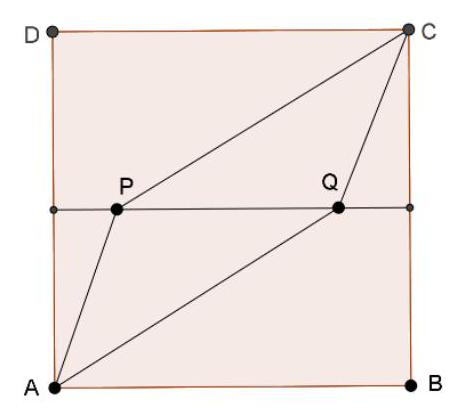
\includegraphics[max width=\textwidth]{2024_11_21_aff3155550b8fa0c078dg-1}
\end{center}

\begin{enumerate}
  \item Oblicz sume: \(\log \left(\operatorname{tg} 1^{\circ}\right)+\log \left(\operatorname{tg} 2^{\circ}\right)+\cdots+\log \left(\operatorname{tg} 88^{\circ}\right)+\log \left(\operatorname{tg} 89^{\circ}\right)\)
  \item Jaka jest maksymalna ilość sfer stycznych do wszystkich płaszczyzn, w których leżą ściany ustalonego czworościanu?
  \item Niech \(f(x)=\prod_{k=1}^{2016}(x+2 k)+\prod_{k=1}^{2016}(x+2 k-1)\). Ile rozwiązań ma równanie \(f(x)=0\) ?\\
Symbol \(\Pi\) to tak zwany iloczyn uogólniony i przykładowo \(\prod_{k=1}^{2016}(x+2 k)\) oznacza iloczyn \((x+2)(x+4) \cdot \ldots \cdot(x+4032)\).
\end{enumerate}

\end{document}